\documentclass{thesis-ekf}
%\documentclass[twoside]{thesis-ekf}
%\documentclass[colorlinks]{thesis-ekf}
\usepackage[T1]{fontenc}
\PassOptionsToPackage{defaults=hu-min}{magyar.ldf}
\usepackage[magyar]{babel}
\usepackage[utf8]{inputenc}
\usepackage{listingsutf8,xcolor,caption,graphicx,amsmath,amssymb,amsthm, url, hulipsum, hyperref}
\footnotestyle{rule=fourth}

\graphicspath{{./kepek/}}

\newtheorem{tetel}{Tétel}[chapter]
\newtheorem{lemma}[tetel]{Lemma}
\theoremstyle{definition}
\newtheorem{definicio}[tetel]{Definíció}
\newtheorem{feladat}[tetel]{Feladat}
\theoremstyle{remark}
\newtheorem{megjegyzes}[tetel]{Megjegyzés}
\newtheorem*{megoldas}{Megoldás}

\begin{document}
\logo{
\includegraphics[width=8cm]{eke-logo.pdf}}
\institute{Matematikai és Informatikai Intézet}
\title{Kliens-szerver kommunikáció\\Android platformon}
\author{Balajti-Tóth Kristóf\\Programtervező Informatikus BSc}
\supervisor{Tajti Tibor\\Egyetemi adjunktus}
\city{Eger}
\date{2019}
\maketitle
\tableofcontents

\chapter*{Bevezetés}
\markboth{Bevezetés}{Bevezetés}
Az szoftver fejlesztés egy nagyon komplex folyamat és rengeteg részletre oda kell figyleni.
Az elkészült programnak hatékonynak, hibamentesnek és gyorsnak kell lennie. Természetesen, mindezt határidőn belül kell teljesíteni.
Sajnos a biztonság nem egy első számú szempont egy megrendelő szemében,csak akkor ha már valami baj történt.
Inkább a gyorsaságon és a folyamatok automatizálásán van a hangsúly, ezért nem  meglepő, hogy a fejlesztés életciklusának tervezési szakaszában kevés figyelem fordul a szoftver biztonságossá tételére.

A statista.com \cite{statista} kutatása szerint 2020-ra több mint 4.78 billió telefon lesz használatban.
Ezzel a cégek is tisztában vannak és tudják, hogy ha még több emberhez szeretnék eljuttatni a szolgáltatásukat, akkor rendelkezniük kell saját mobilos alkalmazással.

A mobilos eszközöket célzó támadások száma hatalmas ütemben nő. Mindez azért lehetséges, mert figyelmen kívül marad a ,,secure coding''-nak nevezett gyakorlat.
Egy alkalmazásnak a sebezhetőségét különböző támadási vektoron is ki lehet aknázni.
Az elején, bennem többek között az a kérdés merült fel, hogy honnan tudható hogy ez alkalmazás ebezhető-e vagy sem.egy kérdés merült fel. Honnann tudhatom, hogy egy adott alkalmazás sebezhető-e vagy sem. A leghatékonyabb módszer ha visszafejtjük a fájl forráskódra. Ezt angolul ,,reverse engineering''-nek nevezik. A visszaállított fájlok olvashatósága nem lesz tökéletes, főleg ha obfuszkált \footnote{Az obfuszkáció célja röviden, hogy megnehezítse a visszafejtett kód olvashatóságát.} kóddal állunk szemben, de egy tapasztalt szem így is kitudja szúrni a gyakori hibákat.

A szakdolgozatomban Android platformra készült telepítő fájlok forrás fájlokká való visszaállításáról írok, valamint bemutatom hogyan valósítható meg a kliens-szerver kommunikáció egy REST~API és egy Androidos alkalmazás segítségével.
A projectet ,,Reverse Droid''-nak neveztem el.

\chapter{Fejlesztői eszközök}\label{eszkozok}

\section{Fejlesztői környezetek}

\subsection{Android Studio}

Az Android Studio jelenleg az egyetlen jól támogatott és minőségi fejlesztői környezet Android fejlesztéshez.
Régebben sok panaszt hallottam az emulátorára, hogy nagyon lassú és körülményes a használata.
Mára már egy pillanat alatt lehet futtatni a programunk és abszolút kényelmes lett a használata.
Rendelkezik APK elemzővel, vizuális felhasználó felület szerkesztővel és intelligens kód szerkesztővel is.
Az egyik kedvenc funkcióm a valós idejű profilozó, ami segítségével megtudjuk nézni valós időben, milyen erőforrásokat használ az alkalmazásuk.
Ez különösen hasznos, ha megakarunk találni egy memória szivárgást vagy egy olyan részt, ami a kelleténél jobban meríti az akkumulátorunk.
Említésre méltó még a flexibilis build rendszere is, a Gradle. Használatával megtehetjük, hogy külön build típusokat hozzunk létre a különböző eszközökre. \cite{androidstudio}

\subsection{Pycharm Professional Edition}

\section{Postman}

\chapter{Platformok}\label{platformok}

\section{A szerver kiválasztása és felépítése}

Olyan szerverre volt szükségem, ami nem túl költséges, de mégis megfelelően testreszabható és gyors tárhelyet biztosít.
A választásom a Digitial Ocean felhő szolgáltatására esett. Az oldal felületén lehetőségünk van több, úgynevezett \emph{droplet}-et létrehozni, amik nem mások mint virtuális szerverek. 
Megadhatjuk milyen disztribúciót szeretnénk telepíteni, jelen esetben én az Ubuntu Linux 18.10-es verzióját telepítettem.

\begin{figure}[!h]
	\centering
	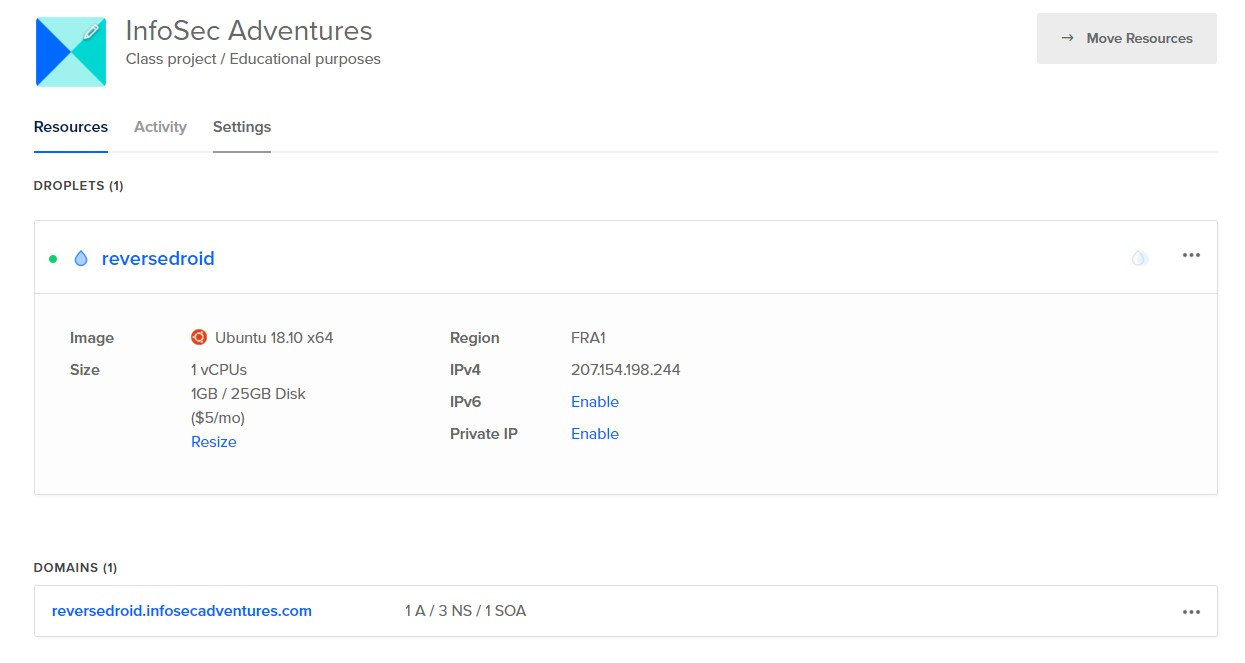
\includegraphics[width=15cm]{kepek/digitalocean}
	\caption{Droplet a Digital Ocean admin felületén.}
	\label{digitalocean}
\end{figure}

A projecthez készítettem egy subdomain-t és telepítés után a droplet IP címét hozzárendeltem ehhez a subdomain-hez.
Ezzel biztosítottam, hogy domain név alapján is elérhető legyen a szerver. Ez a \ref{namecheap} képen jól látható.

\begin{figure}[!h]
	\centering
	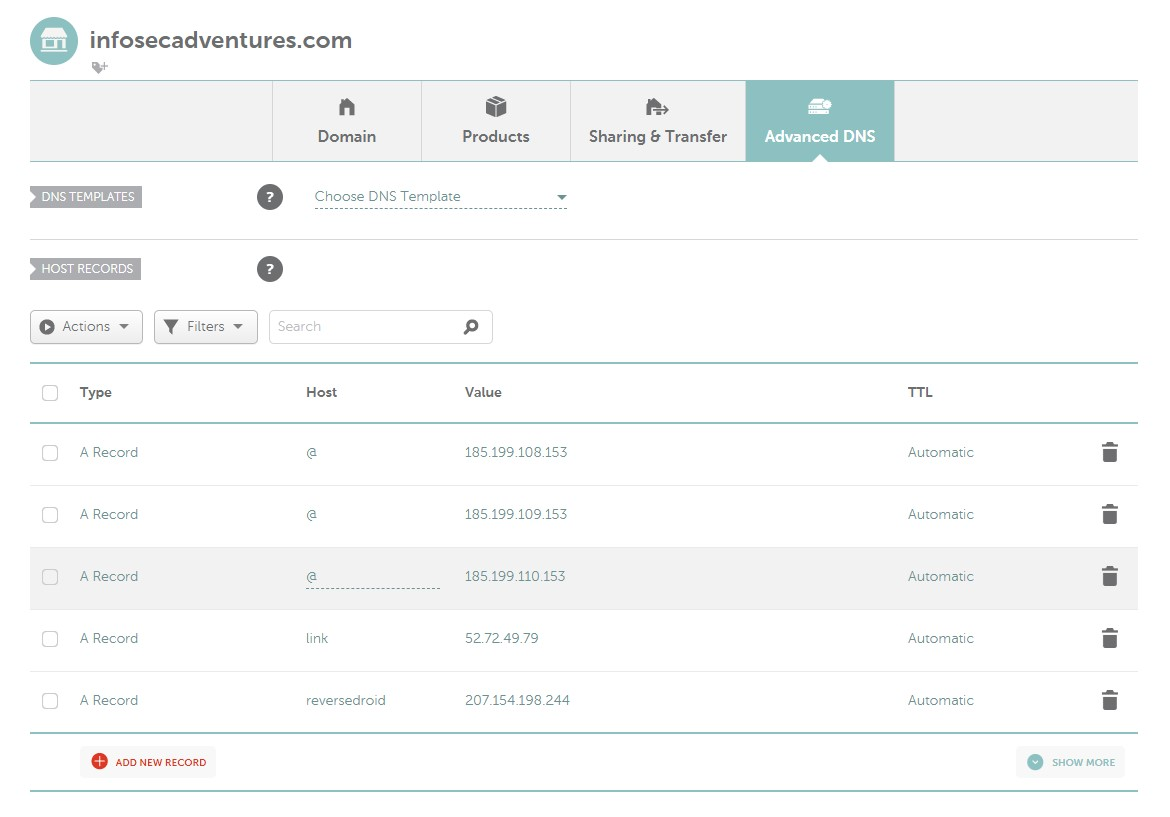
\includegraphics[width=15cm]{kepek/namecheap}
	\caption{DNS rekordok a domain beállításaiban.}
	\label{namecheap}
\end{figure}

A kész projectben nem ezt a folyamatot választottam, hanem a Digital Ocean által nyújtott ,,one-click apps'' menüben egyszerűen kiválasztottam a Docker alkalmazást és az elkészült képfájlt ezen futattam. 
Így automatizálva a szerver telepítésének folyamatát és megspórolva magának a Docker-nek a telepítését és konfigurálását.
Erről még a Szerveren használt technológiák fejezet \nameref{docker} alfejezetében bővebben írok.

\section{Mobil platform választása}

A mobilos operációs rendszerek közül az Androidot választottam. Már korábban sikerült megismerkednem az Android nyújtotta lehetőségekkel és előnyökkel.
A többi mobilos operációs rendszerrel ellentétben az Android nyílt forráskódú és a piac több mint felét uralja.
Ez annak is köszönhető, hogy 2005-ben a Google felvásárolta az Android projectet és azóta ők tartják karban.
A fejlesztő környezete elérhető mind a három fő operációs rendszerre (Linux, macOS, Windows).
Számomra ezek voltak a legnyomósabb érvek a rendszer kiválasztásában.

\chapter{Felhasznált technológiák}\label{technologiak}

\section{Folyamatos integrálás}

A folyamatos integrálás egy extrém programozási gyakorlat.
A folyamatos integrálás arról szól, hogy ha egy feladat elkészült akkor azt egyből beintegráljuk a rendszerbe.
A beintegrálás után természetesen minden egység tesztnek sikeresen le kell futnia.
Több nagy cég is a \emph{CircleCi}-t használja a folyamatos integráláshoz.
Ilyen például a \emph{Facebook}, \emph{Spotify}, \emph{Kickstarter} és a \emph{GoPro}.

\begin{figure}[!h]
	\centering
	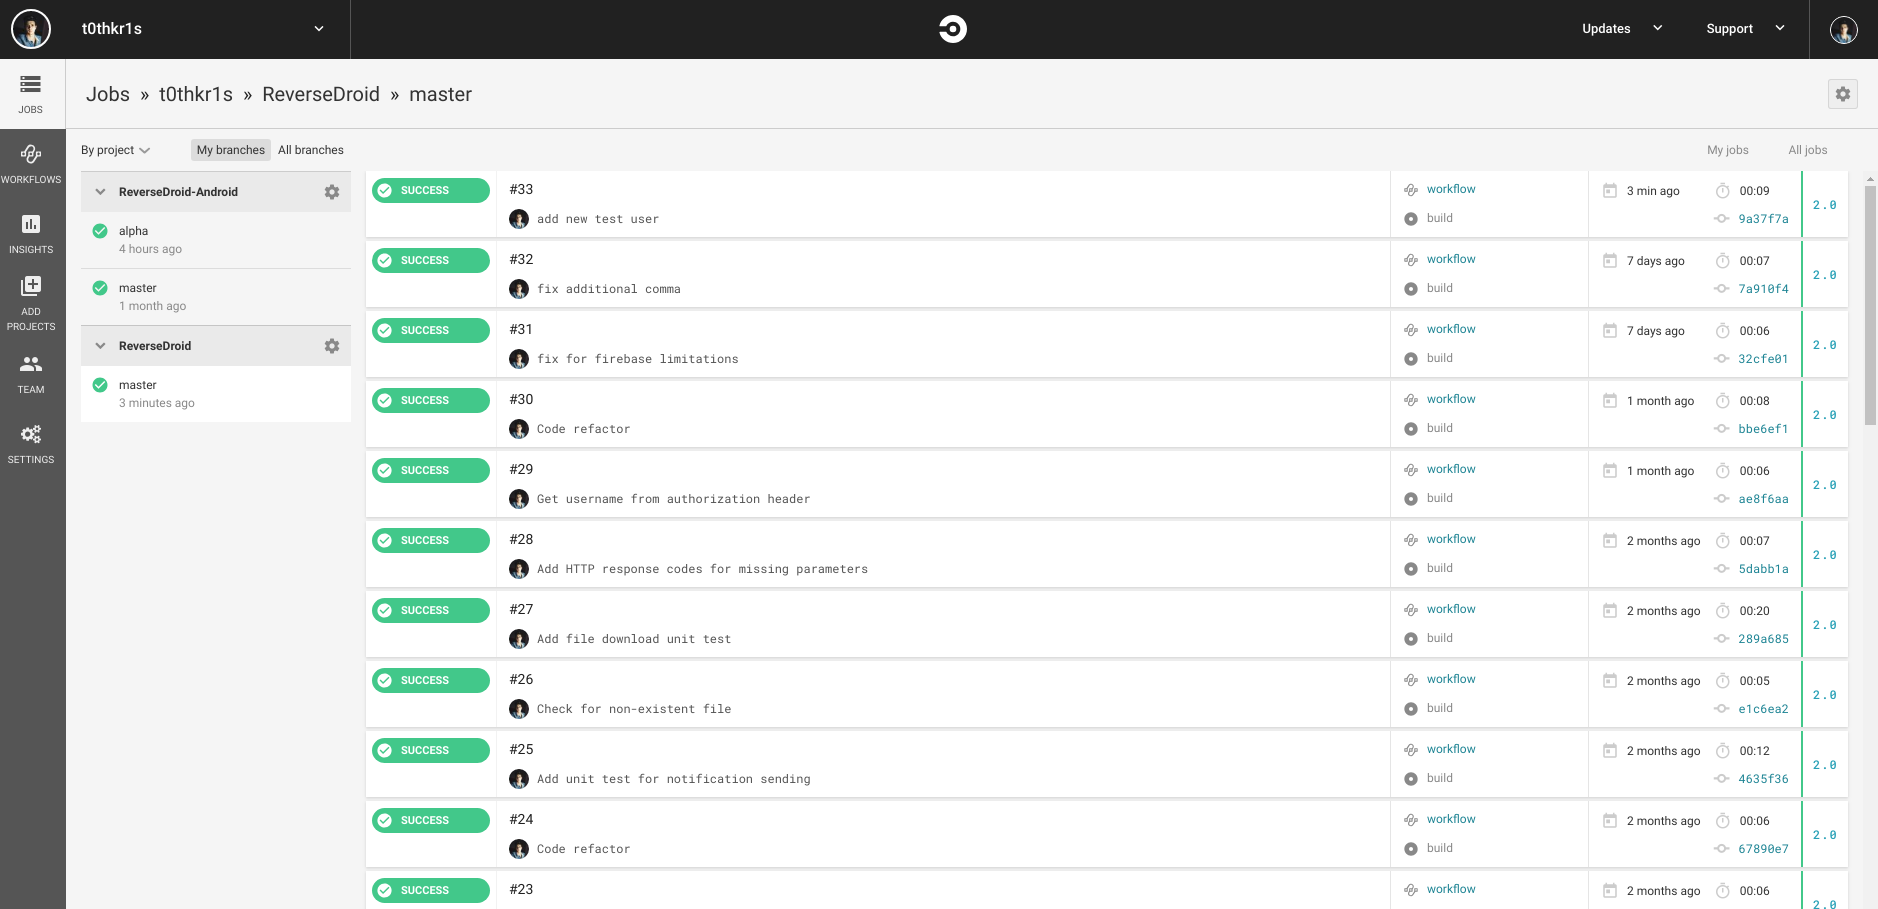
\includegraphics[width=15cm]{kepek/circle_ci}
	\caption{Sikeres project buildek a CircleCi felületén.}
	\label{circleci}
\end{figure}


\section{Verzió kezelés}

Már a project kezdetekor készítettem egy privát Github repository-t, hogy nyomon tudjam követni a változtatásaimat és esetleges hiba esetén visszaállítani egy korábbi verzióra.


\section{Szerveren használt technológiák}

\subsection{Flask}

A szervert a Flask webes mikro keretrendszer felhasználásával készítettem el.
A \emph{LinkedIn} és \emph{Pinteres} is említésre méltó alkalmazások, amik felhasználták ezt a keretrendszert.

\subsection{SQLite}

Az SQLite a legtöbbet használt adatbázis motor a világon. 
Számtalan alkalmazás használja és Android-on is ez az alapértelmezett adatbázis.
Az SQLite nyílt forráskódú, így mindenki nyugodtan használhatja.

\subsection{Docker}\label{docker}

A szerverhez készítettem egy Dockerfile-t és csatoltam a project Github-os repository-ját.
Ezzel elérve, hogy minden egyes változatásnál a Docker Hub újra buildelje a képfájlt.
A folyamat nagyon hasonlít a folyamatos integrálásra.

\begin{figure}[!h]
	\centering
	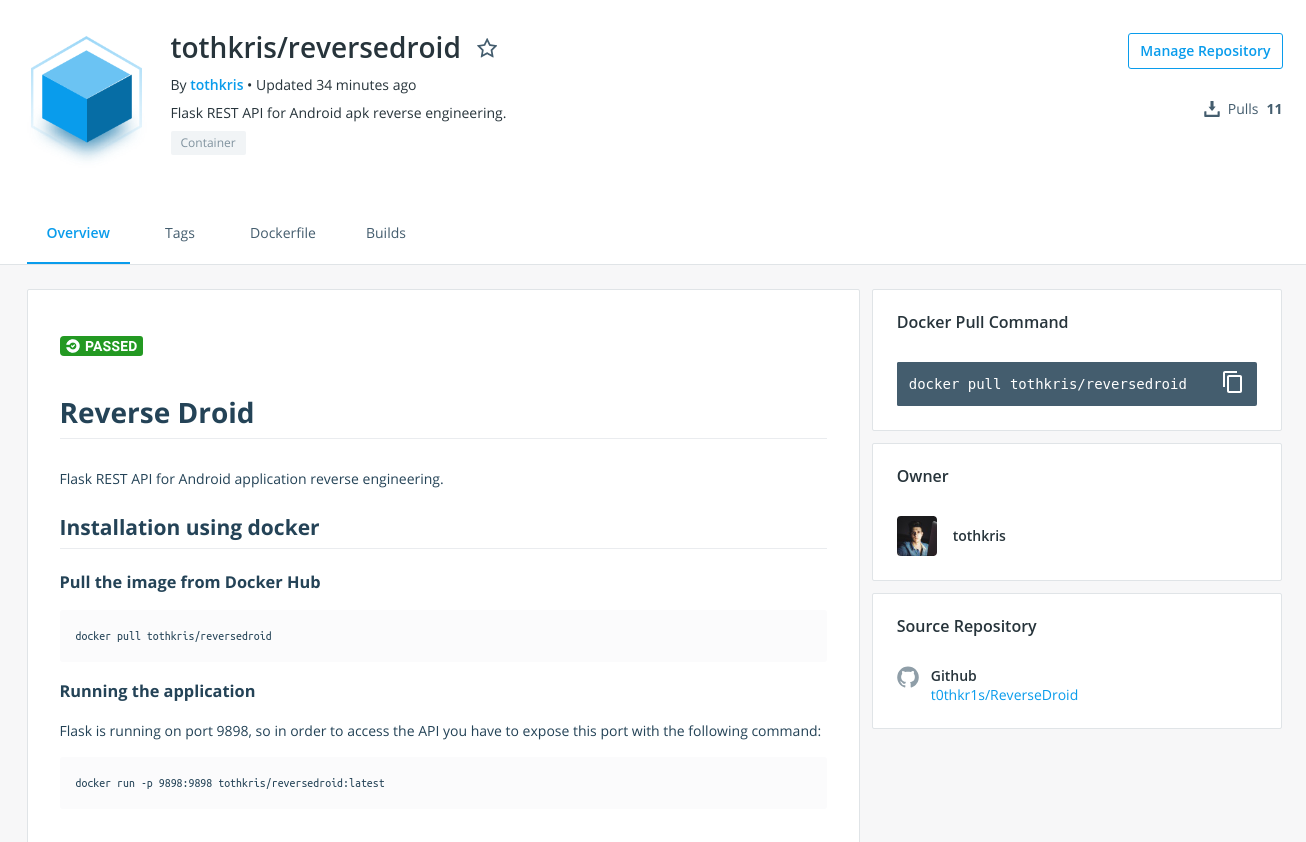
\includegraphics[width=15cm]{kepek/docker_hub}
	\caption{A szerver Docker Hub-on is elérhető.}
	\label{dockerhub}
\end{figure}

\subsection{Tmux}

A Tmux vagy másnéven terminál multiplexer használatával több shell-t lehet futtatni.
Ez még nem is lenne túl nagy segítség, viszont ezt a folyamatot le lehet csatolni majd vissza anélkül, hogy elveszne a tartalom.
Ezen felül biztosítja, hogy a parancsok és azok kimenete kereshetők legyenek.
Az alkalmazás alapvetően a parancssorba írja a bejövő kéréseket és ez egy idő után nehezen követhető.
A Tmux nagy segítségemre volt, mivel lehetőséget adott hogy keressek a kérések között.

\subsection{jd-cmd}

Szükségem volt egy parancs sorból használható Java Decompiler-re is. 

\url{https://github.com/kwart/jd-cmd}

\subsection{Apktool}

\url{https://github.com/iBotPeaches/Apktool}

\subsection{dex2jar}

\url{https://bitbucket.org/pxb1988/dex2jar}

\subsection{JSON}



\section{Androidon használt technológiák}

\subsection{OkHttp3}

\subsection{Okio}

\subsection{Pusher}

\subsection{Firebase Messaging}

\subsection{Room}

\subsection{CodeView}

A forrás kód megjelenítését nem lett volna célszerű nulláról felépíteni, ezért inkább kész megoldások után néztem.
Több megfelelő forrás kód megjelenítő könyvtárat találtam, így funkciók alapján kellett döntenem, hogy melyiket válasszam.

\begin{figure}[!h]
	\centering
	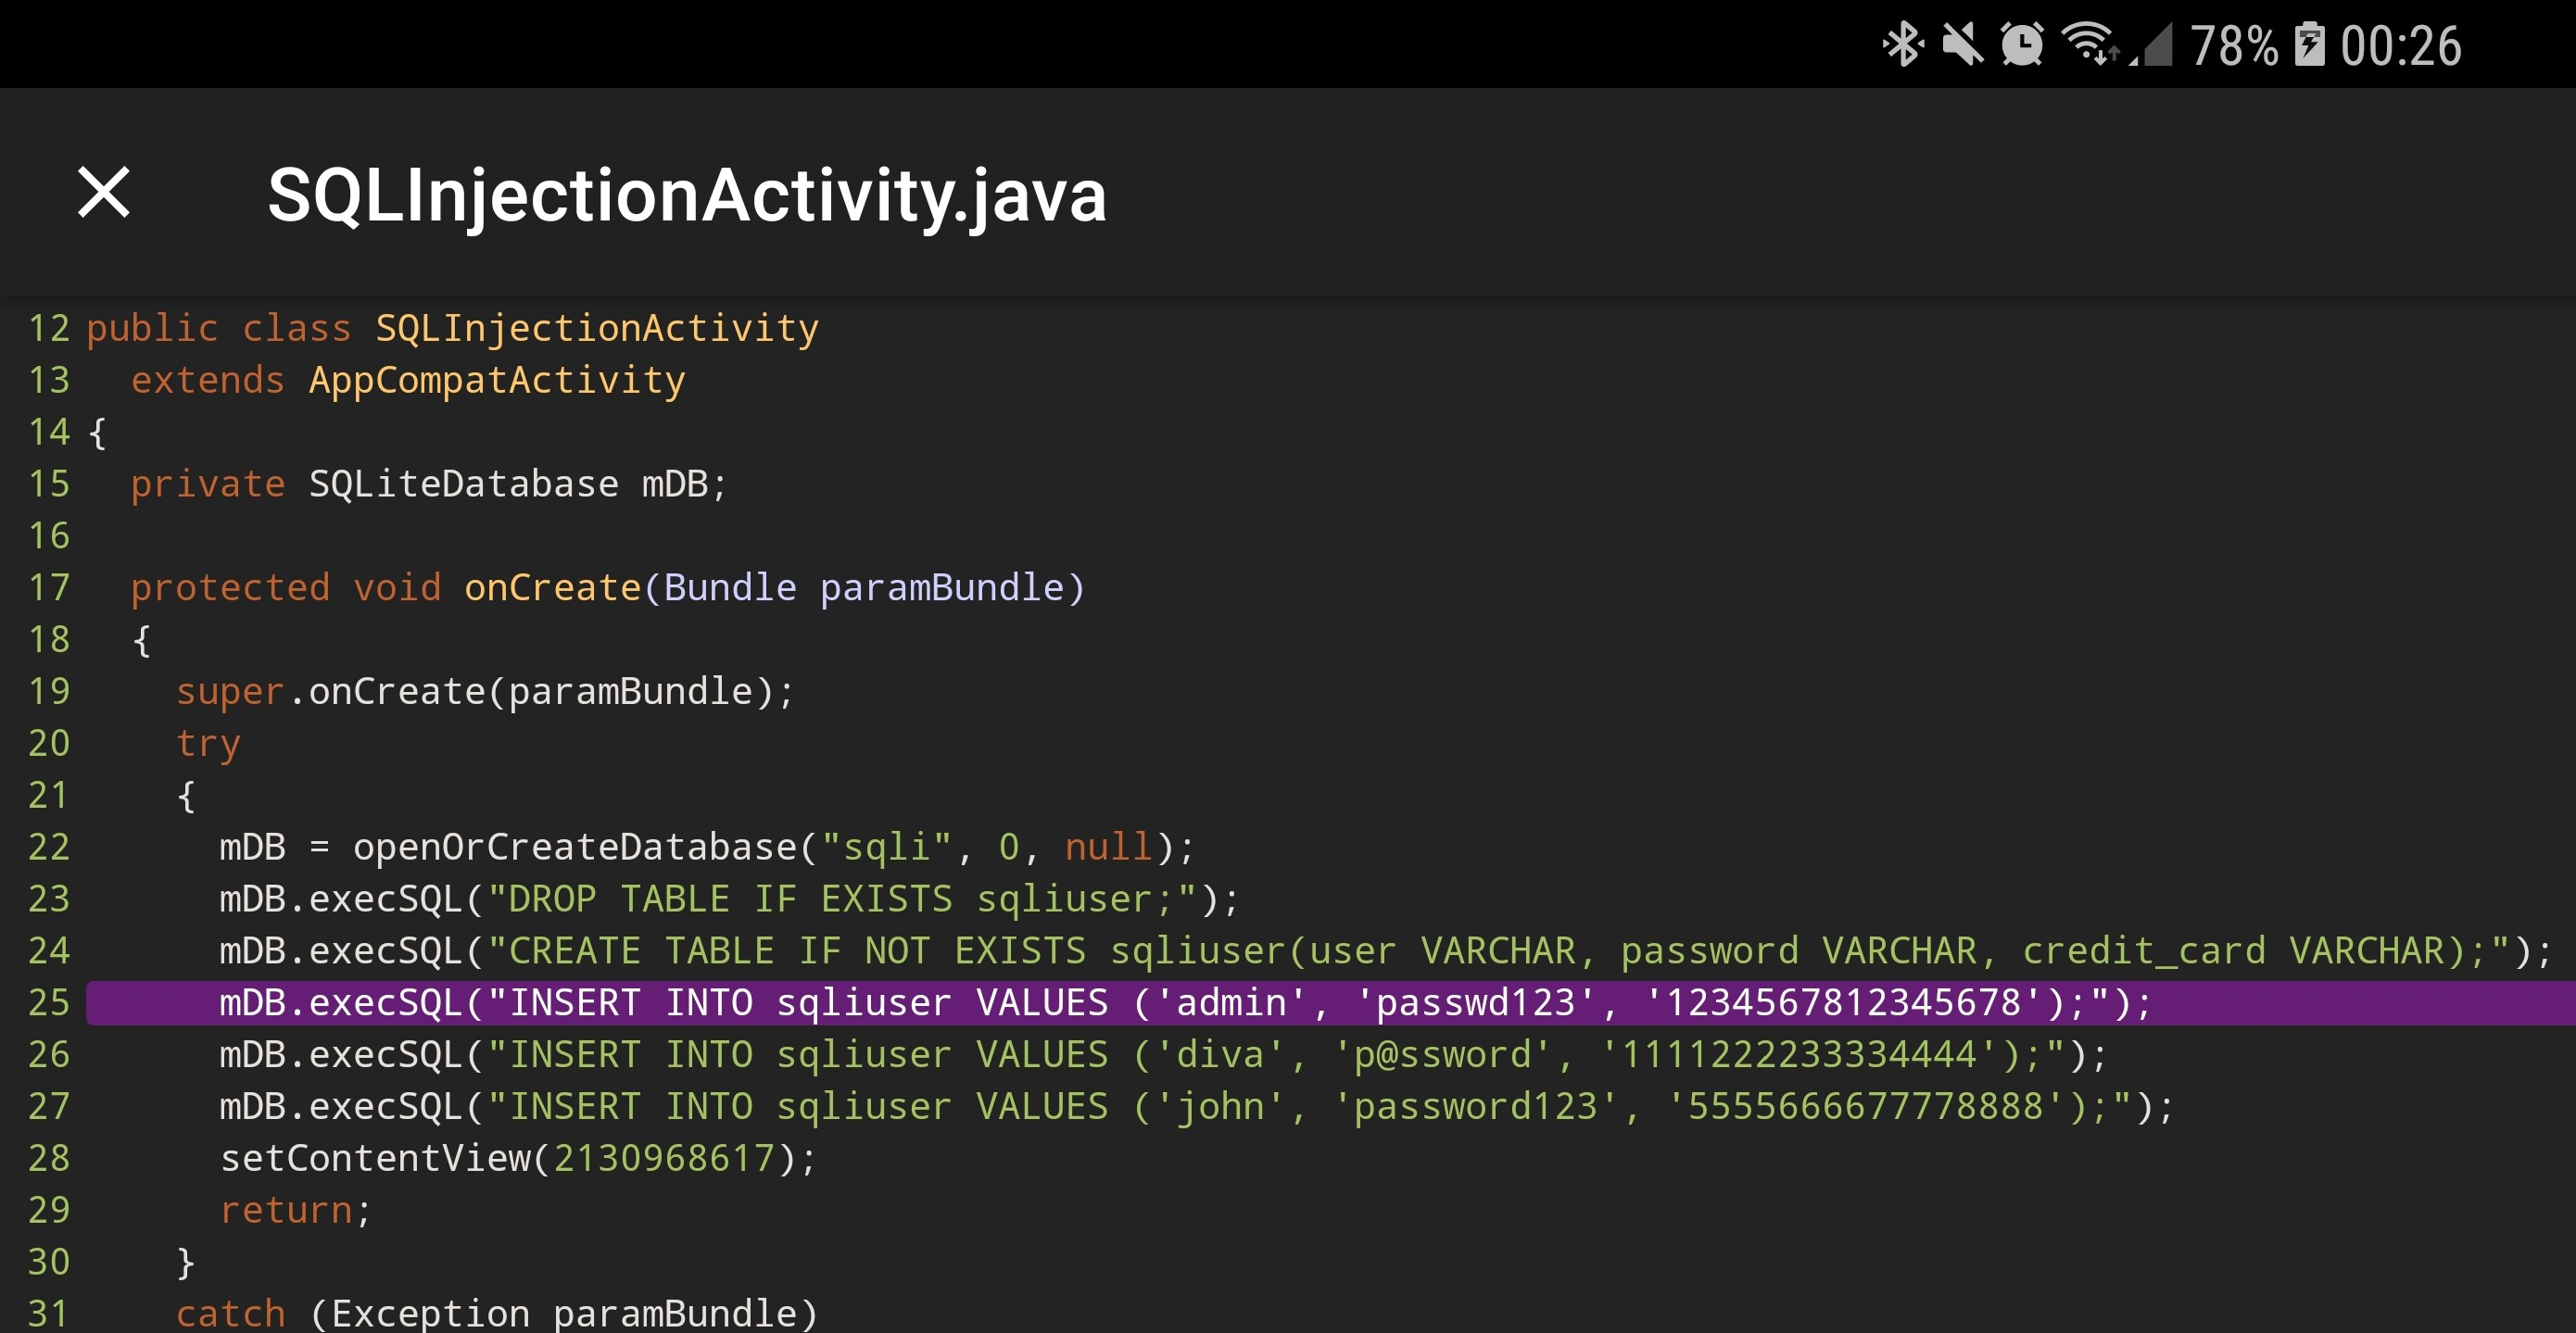
\includegraphics[width=15cm]{kepek/code_view}
	\caption{A vissza fejtett forrás kód megjelenítése.}
	\label{dockerhub}
\end{figure}

\subsection{Espresso}

\subsection{Material Design 2.0}

\chapter{Teszteléshez felhasznált eszközök és források}\label{teszteles}

\subsection{Sérülékeny Android alkalmazások}

A teszteléshez keresnem kellett olyan sérülékeny alkalmazásokat, amelyeken jól lehet demonstrálni a visszafejtést.
Minden alkalmazás, amit itt megemlítek nyílt forrás kódú és kimondottan erre a céltra készítették őket.
Ez azért is jó, mert a visszafejtett kódot össze lehet hasonlítani az eredetivel és megnézni mennyire volt hatékony a visszafejtési folyamat.
A következő lista tartalmazza a teszteléshez felhasznált szándékosan sérülékeny alkalmazásokat.

\begin{itemize}
	\item \href{https://github.com/payatu/diva-android}{Diva}
	\item \href{https://github.com/as0ler/Android-Examples}{Sieve}
	\item \href{https://github.com/htbridge/pivaa}{Pivaa}
	\item \href{https://github.com/t0thkr1s/frida-demo}{Frida}
\end{itemize}

\chapter{Megvalósított funkciók}\label{funkciok}

\chapter{Továbbfejlesztési lehetőségek}\label{lehetosegek}

Úgy gondolom, hogy sokkal nagyobb piaci érték rejlik ebben az alkalmazásban.
A jövőben is szeretném folytatni a fejlesztést.
Szeretnék több figyelmet fordítani az biztonságra és hatékonyságra.
Gondolok itt a biztonságos kommunikációra TLS-es keresztül és a harmadik féltől származó könyvtárak csökkentésére.
A kód visszafejtése végén egy összegző report is hasznos lehet a felhasználó számára, ami tartalmazhatja a feldolgozott fájlok számát.

\chapter{Tapasztalatok}\label{tapasztalatok}

Úgy érzem elértem a célom ezzel a projecttel és sokat sikerült tanulnom a folyamatban.
Új technológiákat ismertem meg és használtam.
Természetesen nem volt minden magától értetődő és jó pár nehézséggel is találkoztam.


\begin{thebibliography}{1}
\bibitem{statista} \textsc{ONLINE}: Number of mobile phone users worldwide from 2015 to 2020, \url{https://www.statista.com/statistics/274774/forecast-of-mobile-phone-users-worldwide}
\bibitem{androidstudio} \textsc{ONLINE}: Everything you need to build on Android \url{https://developer.android.com/studio/features.html}
\end{thebibliography}
\end{document}
